% Options for packages loaded elsewhere
\PassOptionsToPackage{unicode}{hyperref}
\PassOptionsToPackage{hyphens}{url}
%
\documentclass[
  letterpaper,
  oneside,
  open=any]{scrbook}

\usepackage{amsmath,amssymb}
\usepackage{lmodern}
\usepackage{iftex}
\ifPDFTeX
  \usepackage[T1]{fontenc}
  \usepackage[utf8]{inputenc}
  \usepackage{textcomp} % provide euro and other symbols
\else % if luatex or xetex
  \usepackage{unicode-math}
  \defaultfontfeatures{Scale=MatchLowercase}
  \defaultfontfeatures[\rmfamily]{Ligatures=TeX,Scale=1}
\fi
% Use upquote if available, for straight quotes in verbatim environments
\IfFileExists{upquote.sty}{\usepackage{upquote}}{}
\IfFileExists{microtype.sty}{% use microtype if available
  \usepackage[]{microtype}
  \UseMicrotypeSet[protrusion]{basicmath} % disable protrusion for tt fonts
}{}
\makeatletter
\@ifundefined{KOMAClassName}{% if non-KOMA class
  \IfFileExists{parskip.sty}{%
    \usepackage{parskip}
  }{% else
    \setlength{\parindent}{0pt}
    \setlength{\parskip}{6pt plus 2pt minus 1pt}}
}{% if KOMA class
  \KOMAoptions{parskip=half}}
\makeatother
\usepackage{xcolor}
\setlength{\emergencystretch}{3em} % prevent overfull lines
\setcounter{secnumdepth}{5}
% Make \paragraph and \subparagraph free-standing
\ifx\paragraph\undefined\else
  \let\oldparagraph\paragraph
  \renewcommand{\paragraph}[1]{\oldparagraph{#1}\mbox{}}
\fi
\ifx\subparagraph\undefined\else
  \let\oldsubparagraph\subparagraph
  \renewcommand{\subparagraph}[1]{\oldsubparagraph{#1}\mbox{}}
\fi
\usepackage{color}
\usepackage{fancyvrb}
\newcommand{\VerbBar}{|}
\newcommand{\VERB}{\Verb[commandchars=\\\{\}]}
\DefineVerbatimEnvironment{Highlighting}{Verbatim}{commandchars=\\\{\}}
% Add ',fontsize=\small' for more characters per line
\usepackage{framed}
\definecolor{shadecolor}{RGB}{241,243,245}
\newenvironment{Shaded}{\begin{snugshade}}{\end{snugshade}}
\newcommand{\AlertTok}[1]{\textcolor[rgb]{0.68,0.00,0.00}{#1}}
\newcommand{\AnnotationTok}[1]{\textcolor[rgb]{0.37,0.37,0.37}{#1}}
\newcommand{\AttributeTok}[1]{\textcolor[rgb]{0.40,0.45,0.13}{#1}}
\newcommand{\BaseNTok}[1]{\textcolor[rgb]{0.68,0.00,0.00}{#1}}
\newcommand{\BuiltInTok}[1]{\textcolor[rgb]{0.00,0.23,0.31}{#1}}
\newcommand{\CharTok}[1]{\textcolor[rgb]{0.13,0.47,0.30}{#1}}
\newcommand{\CommentTok}[1]{\textcolor[rgb]{0.37,0.37,0.37}{#1}}
\newcommand{\CommentVarTok}[1]{\textcolor[rgb]{0.37,0.37,0.37}{\textit{#1}}}
\newcommand{\ConstantTok}[1]{\textcolor[rgb]{0.56,0.35,0.01}{#1}}
\newcommand{\ControlFlowTok}[1]{\textcolor[rgb]{0.00,0.23,0.31}{#1}}
\newcommand{\DataTypeTok}[1]{\textcolor[rgb]{0.68,0.00,0.00}{#1}}
\newcommand{\DecValTok}[1]{\textcolor[rgb]{0.68,0.00,0.00}{#1}}
\newcommand{\DocumentationTok}[1]{\textcolor[rgb]{0.37,0.37,0.37}{\textit{#1}}}
\newcommand{\ErrorTok}[1]{\textcolor[rgb]{0.68,0.00,0.00}{#1}}
\newcommand{\ExtensionTok}[1]{\textcolor[rgb]{0.00,0.23,0.31}{#1}}
\newcommand{\FloatTok}[1]{\textcolor[rgb]{0.68,0.00,0.00}{#1}}
\newcommand{\FunctionTok}[1]{\textcolor[rgb]{0.28,0.35,0.67}{#1}}
\newcommand{\ImportTok}[1]{\textcolor[rgb]{0.00,0.46,0.62}{#1}}
\newcommand{\InformationTok}[1]{\textcolor[rgb]{0.37,0.37,0.37}{#1}}
\newcommand{\KeywordTok}[1]{\textcolor[rgb]{0.00,0.23,0.31}{#1}}
\newcommand{\NormalTok}[1]{\textcolor[rgb]{0.00,0.23,0.31}{#1}}
\newcommand{\OperatorTok}[1]{\textcolor[rgb]{0.37,0.37,0.37}{#1}}
\newcommand{\OtherTok}[1]{\textcolor[rgb]{0.00,0.23,0.31}{#1}}
\newcommand{\PreprocessorTok}[1]{\textcolor[rgb]{0.68,0.00,0.00}{#1}}
\newcommand{\RegionMarkerTok}[1]{\textcolor[rgb]{0.00,0.23,0.31}{#1}}
\newcommand{\SpecialCharTok}[1]{\textcolor[rgb]{0.37,0.37,0.37}{#1}}
\newcommand{\SpecialStringTok}[1]{\textcolor[rgb]{0.13,0.47,0.30}{#1}}
\newcommand{\StringTok}[1]{\textcolor[rgb]{0.13,0.47,0.30}{#1}}
\newcommand{\VariableTok}[1]{\textcolor[rgb]{0.07,0.07,0.07}{#1}}
\newcommand{\VerbatimStringTok}[1]{\textcolor[rgb]{0.13,0.47,0.30}{#1}}
\newcommand{\WarningTok}[1]{\textcolor[rgb]{0.37,0.37,0.37}{\textit{#1}}}

\providecommand{\tightlist}{%
  \setlength{\itemsep}{0pt}\setlength{\parskip}{0pt}}\usepackage{longtable,booktabs,array}
\usepackage{calc} % for calculating minipage widths
% Correct order of tables after \paragraph or \subparagraph
\usepackage{etoolbox}
\makeatletter
\patchcmd\longtable{\par}{\if@noskipsec\mbox{}\fi\par}{}{}
\makeatother
% Allow footnotes in longtable head/foot
\IfFileExists{footnotehyper.sty}{\usepackage{footnotehyper}}{\usepackage{footnote}}
\makesavenoteenv{longtable}
\usepackage{graphicx}
\makeatletter
\def\maxwidth{\ifdim\Gin@nat@width>\linewidth\linewidth\else\Gin@nat@width\fi}
\def\maxheight{\ifdim\Gin@nat@height>\textheight\textheight\else\Gin@nat@height\fi}
\makeatother
% Scale images if necessary, so that they will not overflow the page
% margins by default, and it is still possible to overwrite the defaults
% using explicit options in \includegraphics[width, height, ...]{}
\setkeys{Gin}{width=\maxwidth,height=\maxheight,keepaspectratio}
% Set default figure placement to htbp
\makeatletter
\def\fps@figure{htbp}
\makeatother
\newlength{\cslhangindent}
\setlength{\cslhangindent}{1.5em}
\newlength{\csllabelwidth}
\setlength{\csllabelwidth}{3em}
\newlength{\cslentryspacingunit} % times entry-spacing
\setlength{\cslentryspacingunit}{\parskip}
\newenvironment{CSLReferences}[2] % #1 hanging-ident, #2 entry spacing
 {% don't indent paragraphs
  \setlength{\parindent}{0pt}
  % turn on hanging indent if param 1 is 1
  \ifodd #1
  \let\oldpar\par
  \def\par{\hangindent=\cslhangindent\oldpar}
  \fi
  % set entry spacing
  \setlength{\parskip}{#2\cslentryspacingunit}
 }%
 {}
\usepackage{calc}
\newcommand{\CSLBlock}[1]{#1\hfill\break}
\newcommand{\CSLLeftMargin}[1]{\parbox[t]{\csllabelwidth}{#1}}
\newcommand{\CSLRightInline}[1]{\parbox[t]{\linewidth - \csllabelwidth}{#1}\break}
\newcommand{\CSLIndent}[1]{\hspace{\cslhangindent}#1}

\makeatletter
\makeatother
\makeatletter
\@ifpackageloaded{bookmark}{}{\usepackage{bookmark}}
\makeatother
\makeatletter
\@ifpackageloaded{caption}{}{\usepackage{caption}}
\AtBeginDocument{%
\ifdefined\contentsname
  \renewcommand*\contentsname{Table of contents}
\else
  \newcommand\contentsname{Table of contents}
\fi
\ifdefined\listfigurename
  \renewcommand*\listfigurename{List of Figures}
\else
  \newcommand\listfigurename{List of Figures}
\fi
\ifdefined\listtablename
  \renewcommand*\listtablename{List of Tables}
\else
  \newcommand\listtablename{List of Tables}
\fi
\ifdefined\figurename
  \renewcommand*\figurename{Figure}
\else
  \newcommand\figurename{Figure}
\fi
\ifdefined\tablename
  \renewcommand*\tablename{Table}
\else
  \newcommand\tablename{Table}
\fi
}
\@ifpackageloaded{float}{}{\usepackage{float}}
\floatstyle{ruled}
\@ifundefined{c@chapter}{\newfloat{codelisting}{h}{lop}}{\newfloat{codelisting}{h}{lop}[chapter]}
\floatname{codelisting}{Listing}
\newcommand*\listoflistings{\listof{codelisting}{List of Listings}}
\makeatother
\makeatletter
\@ifpackageloaded{caption}{}{\usepackage{caption}}
\@ifpackageloaded{subcaption}{}{\usepackage{subcaption}}
\makeatother
\makeatletter
\@ifpackageloaded{tcolorbox}{}{\usepackage[many]{tcolorbox}}
\makeatother
\makeatletter
\@ifundefined{shadecolor}{\definecolor{shadecolor}{rgb}{.97, .97, .97}}
\makeatother
\makeatletter
\makeatother

\usepackage{hyphenat}
\usepackage{ifthen}
\usepackage{calc}
\usepackage{calculator}



\usepackage{graphicx}
\usepackage{geometry}
\usepackage{afterpage}
\usepackage{tikz}
\usetikzlibrary{calc}
\usetikzlibrary{fadings}
\usepackage[pagecolor=none]{pagecolor}



% Set the titlepage font families







% Set the coverpage font families





\ifLuaTeX
  \usepackage{selnolig}  % disable illegal ligatures
\fi
\IfFileExists{bookmark.sty}{\usepackage{bookmark}}{\usepackage{hyperref}}
\IfFileExists{xurl.sty}{\usepackage{xurl}}{} % add URL line breaks if available
\urlstyle{same} % disable monospaced font for URLs
\hypersetup{
  pdftitle={NOAA quarto book},
  pdfauthor={Jane Doe; Eva Nováková; Matti Meikäläinen},
  hidelinks,
  pdfcreator={LaTeX via pandoc}}

\title{NOAA quarto book}
\author{Jane Doe \and Eva Nováková \and Matti Meikäläinen}
\date{}

\begin{document}
%%%%% begin titlepage extension code

  \begin{frontmatter}

\begin{titlepage}

%%% TITLE PAGE START

% Set up alignment commands
%Page
\newcommand{\titlepagepagealign}{
\ifthenelse{\equal{left}{right}}{\raggedleft}{}
\ifthenelse{\equal{left}{center}}{\centering}{}
\ifthenelse{\equal{left}{left}}{\raggedright}{}
}


\newcommand{\titleandsubtitle}{
% Title and subtitle
{{\Large{\nohyphens{NOAA quarto book}}}\par
}%
}
\newcommand{\titlepagetitleblock}{
\titleandsubtitle
}

\newcommand{\authorstyle}[1]{{#1}}

\newcommand{\affiliationstyle}[1]{{#1}}

\newcommand{\titlepageauthorblock}{
\authorstyle{Jane Doe{\textsuperscript{1}},  Eva
Nováková{\textsuperscript{2}} and Matti
Meikäläinen{\textsuperscript{3}}%

}}

\newcommand{\titlepageaffiliationblock}{
\hangindent=1em
\hangafter=1
\affiliationstyle{
{1}.~NOAA Fisheres, Northwest Fisheries Science Center
\par\hangindent=1em\hangafter=1%
{2}.~NOAA Fisheries, West Coast Regional Office
\par\hangindent=1em\hangafter=1%
{3}.~NOAA Fisheries, Southwest Fisheries Science Center


\vspace{1\baselineskip} 
}
}
\newcommand{\headerstyled}{%
{}
}
\newcommand{\footerstyled}{%
{}
}
\newcommand{\datestyled}{%
{}
}


\newcommand{\titlepageheaderblock}{\headerstyled}

\newcommand{\titlepagefooterblock}{
\footerstyled
}

\newcommand{\titlepagedateblock}{
\datestyled
}

%set up blocks so user can specify order
\newcommand{\titleblock}{{

{\titlepagetitleblock}
}

\vspace{4\baselineskip}
}

\newcommand{\authorblock}{{\titlepageauthorblock}

\vspace{2\baselineskip}
}

\newcommand{\affiliationblock}{{\titlepageaffiliationblock}

\vspace{2\baselineskip}
}

\newcommand{\logoblock}{}

\newcommand{\footerblock}{}

\newcommand{\dateblock}{}

\newcommand{\headerblock}{}

\thispagestyle{empty} % no page numbers on titlepages


\newlength{\minipagewidth}
\setlength{\minipagewidth}{\textwidth}
\raggedright % single minipage
% [position of box][box height][inner position]{width}
% [s] means stretch out vertically; assuming there is a vfill
\begin{minipage}[b][\textheight][s]{\minipagewidth}
\titlepagepagealign
\headerblock

\titleblock

\authorblock

\affiliationblock

\vfill

\logoblock

\footerblock
\par

\end{minipage}\ifthenelse{\equal{}{right} \OR \equal{}{leftright} }{
\hspace{\B}
\vrulecode}{}
\clearpage
%%% TITLE PAGE END
\end{titlepage}
\setcounter{page}{1}
\end{frontmatter}

%%%%% end titlepage extension code\ifdefined\Shaded\renewenvironment{Shaded}{\begin{tcolorbox}[frame hidden, borderline west={3pt}{0pt}{shadecolor}, enhanced, breakable, boxrule=0pt, sharp corners, interior hidden]}{\end{tcolorbox}}\fi

\renewcommand*\contentsname{Table of contents}
{
\setcounter{tocdepth}{2}
\tableofcontents
}
\mainmatter
\bookmarksetup{startatroot}

\hypertarget{rm2024-5}{%
\chapter{RM2024-5}\label{rm2024-5}}

Quarto enables you to weave together content and executable code into a
finished document. To learn more about Quarto see
\url{https://quarto.org}.

\begin{verbatim}
[1] 2
\end{verbatim}

\bookmarksetup{startatroot}

\hypertarget{set-up}{%
\chapter{Set-up}\label{set-up}}

This is a template for a simple Quarto book output to html, PDF or docx
format. It includes a GitHub Action that will build the website
automatically when you make changes to the files. The NOAA palette and
fonts has been added to \texttt{theme.scss}. The webpage will be on the
\texttt{gh-pages} branch. Serving the website files from this branch is
a common way to keep all the website files from cluttering your main
branch.

The GitHub Action installs R so you can have R code in your qmd or Rmd
files. Note, you do not need to make changes to your Rmd files unless
your need Quarto features like cross-references.

\begin{itemize}
\item
  Click the green ``use template'' button to make a repository with this
  content. Make sure to make your repo public (since GitHub Pages
  doesn't work on private repos unless you have a paid account) and
  check box to include all the branches (so that you get the gh-pages
  branch).
\item
  Turn on GitHub Pages under Settings \textgreater{} Pages . You will
  set pages to be made from the gh-pages branch and root directory.
\item
  Turn on GitHub Actions under Settings \textgreater{} Actions
  \textgreater{} General
\item
  Edit the repo description and Readme to add a link to the webpage.
  When you edit the description, you will see the link url in the url
  box or you can click on the Actions tab or the Settings \textgreater{}
  Pages page to find the url.
\end{itemize}

\bookmarksetup{startatroot}

\hypertarget{customize}{%
\chapter{Customize}\label{customize}}

Edit the qmd or md files in the \texttt{content} folder. qmd files can
include code (R, Python, Julia) and lots of Quarto markdown bells and
whistles (like call-outs, cross-references, auto-citations and much
more).

Each page should start with

\begin{verbatim}
---
title: your title
---
\end{verbatim}

and the first header will be the 2nd level, so \texttt{\#\#}. Note,
there are situations where you leave off

\begin{verbatim}
---
title: your title
---
\end{verbatim}

and start the qmd file with a level header \texttt{\#}, but if using the
default title yaml (in the \texttt{-\/-\/-} fence) is a good habit since
it makes it easy for Quarto convert your qmd file to other formats (like
into a presentation).

\hypertarget{add-your-pages-the-project}{%
\section{Add your pages the project}\label{add-your-pages-the-project}}

\begin{itemize}
\tightlist
\item
  Add the files to \texttt{\_quarto.yml}
\end{itemize}

\bookmarksetup{startatroot}

\hypertarget{customization}{%
\chapter{Customization}\label{customization}}

Quarto allow many bells and whistles to make nice output. Read the
documentation here \href{https://quarto.org/docs/guide/}{Quarto
documentation}.

\hypertarget{examples}{%
\section{Examples}\label{examples}}

Looking at other people's Quarto code is a great way to figure out how
to do stuff. Most will have a link to a GitHub repo where you can see
the raw code. Look for a link to edit page or see source code. This will
usually be on the right. Or look for the GitHub icon somewhere.

\begin{itemize}
\tightlist
\item
  \href{https://quarto.org/docs/gallery/}{Quarto gallery}
\item
  \href{https://nmfs-openscapes.github.io/}{nmfs-openscapes}
\item
  \href{https://thefaylab.github.io/lab-manual/}{Faye lab manual}
\item
  \href{https://nmfs-opensci.github.io/quarto_titlepages/}{quarto-titlepages}
  Note the link to edit is broken. Go to repo and look in
  \texttt{documentation} directory.
\end{itemize}

\bookmarksetup{startatroot}

\hypertarget{rendering}{%
\chapter{Rendering}\label{rendering}}

The repo includes a GitHub Action that will render (build) the website
automatically when you make changes to the files. It will be pushed to
the \texttt{gh-pages} branch.

But when you are developing your content, you will want to render it
locally.

Have you updated RStudio since about August 2022? No? Then update to a
newer version of RStudio. In general, you want to keep RStudio updated
and it is required to have a recent version to use Quarto.

\hypertarget{step-2.-clone-and-create-rstudio-project}{%
\section{Step 2. Clone and create RStudio
project}\label{step-2.-clone-and-create-rstudio-project}}

First, clone the repo onto your local computer. How? You can click File
\textgreater{} New Project and then select ``Version Control''. Paste in
the url of the repository. That will clone the repo on to your local
computer. When you make changes, you will need to push those up.

\hypertarget{step-3.-render-within-rstudio}{%
\section{Step 3. Render within
RStudio}\label{step-3.-render-within-rstudio}}

RStudio will recognize that this is a Quarto project by the presence of
the \texttt{\_quarto.yml} file and will see the ``Build'' tab. Click the
``Render website'' button to render to the \texttt{\_site} folder.

\textbf{Previewing:} You can either click \texttt{index.html} in the
\texttt{\_site} folder and specify ``preview in browser'' or set up
RStudio to preview to the viewer panel. To do the latter, go to Tools
\textgreater{} Global Options \textgreater{} R Markdown. Then select
``Show output preview in: Viewer panel''.

\bookmarksetup{startatroot}

\hypertarget{r-markdown}{%
\chapter{R Markdown}\label{r-markdown}}

You can include R Markdown files in your project.

This is an R Markdown document. Markdown is a simple formatting syntax
for authoring HTML, PDF, and MS Word documents. For more details on
using R Markdown see \url{http://rmarkdown.rstudio.com}.

When you click the \textbf{Knit} button a document will be generated
that includes both content as well as the output of any embedded R code
chunks within the document. You can embed an R code chunk like this:

\begin{Shaded}
\begin{Highlighting}[]
\FunctionTok{summary}\NormalTok{(cars)}
\end{Highlighting}
\end{Shaded}

\begin{verbatim}
     speed           dist       
 Min.   : 4.0   Min.   :  2.00  
 1st Qu.:12.0   1st Qu.: 26.00  
 Median :15.0   Median : 36.00  
 Mean   :15.4   Mean   : 42.98  
 3rd Qu.:19.0   3rd Qu.: 56.00  
 Max.   :25.0   Max.   :120.00  
\end{verbatim}

\hypertarget{including-plots}{%
\section{Including Plots}\label{including-plots}}

You can also embed plots and reference them, like so
Figure~\ref{fig-pressure}.

\begin{figure}

{\centering 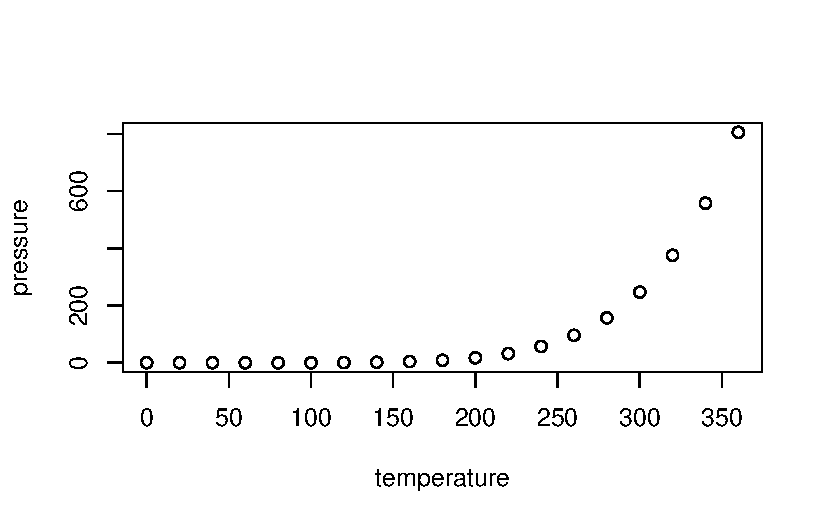
\includegraphics{content/rmarkdown_files/figure-pdf/fig-pressure-1.pdf}

}

\caption{\label{fig-pressure}Plot of pressure}

\end{figure}

Note that the \texttt{echo\ =\ FALSE} parameter was added to the code
chunk to prevent printing of the R code that generated the plot.

\hypertarget{including-tables}{%
\section{Including Tables}\label{including-tables}}

You can also embed tables and reference them with Table~\ref{tbl-iris}.

\begin{Shaded}
\begin{Highlighting}[]
\FunctionTok{library}\NormalTok{(knitr)}
\FunctionTok{kable}\NormalTok{(}\FunctionTok{head}\NormalTok{(iris))}
\end{Highlighting}
\end{Shaded}

\hypertarget{tbl-iris}{}
\begin{longtable}[]{@{}rrrrl@{}}
\caption{\label{tbl-iris}Iris Data}\tabularnewline
\toprule()
Sepal.Length & Sepal.Width & Petal.Length & Petal.Width & Species \\
\midrule()
\endfirsthead
\toprule()
Sepal.Length & Sepal.Width & Petal.Length & Petal.Width & Species \\
\midrule()
\endhead
5.1 & 3.5 & 1.4 & 0.2 & setosa \\
4.9 & 3.0 & 1.4 & 0.2 & setosa \\
4.7 & 3.2 & 1.3 & 0.2 & setosa \\
4.6 & 3.1 & 1.5 & 0.2 & setosa \\
5.0 & 3.6 & 1.4 & 0.2 & setosa \\
5.4 & 3.9 & 1.7 & 0.4 & setosa \\
\bottomrule()
\end{longtable}

\bookmarksetup{startatroot}

\hypertarget{rendering-with-code}{%
\chapter{Rendering with Code}\label{rendering-with-code}}

You can have code (R, Python or Julia) in your qmd file. You will need
to have these installed on your local computer, but presumably you do
already if you are adding code to your qmd files.

\begin{Shaded}
\begin{Highlighting}[]
\NormalTok{x }\OtherTok{\textless{}{-}} \FunctionTok{c}\NormalTok{(}\DecValTok{5}\NormalTok{, }\DecValTok{15}\NormalTok{, }\DecValTok{25}\NormalTok{, }\DecValTok{35}\NormalTok{, }\DecValTok{45}\NormalTok{, }\DecValTok{55}\NormalTok{)}
\NormalTok{y }\OtherTok{\textless{}{-}} \FunctionTok{c}\NormalTok{(}\DecValTok{5}\NormalTok{, }\DecValTok{20}\NormalTok{, }\DecValTok{14}\NormalTok{, }\DecValTok{32}\NormalTok{, }\DecValTok{22}\NormalTok{, }\DecValTok{38}\NormalTok{)}
\FunctionTok{lm}\NormalTok{(x }\SpecialCharTok{\textasciitilde{}}\NormalTok{ y)}
\end{Highlighting}
\end{Shaded}

\begin{verbatim}

Call:
lm(formula = x ~ y)

Coefficients:
(Intercept)            y  
      1.056        1.326  
\end{verbatim}

You will need to change the GitHub Action in \texttt{.github/workflows}
to install these and any needed packages in order for GitHub to be able
to render your webpage. The GitHub Action install R since I used that in
\texttt{code.qmd}. If you use Python or Julia instead, then you will
need to update the GitHub Action to install those.

If getting the GitHub Action to work is too much hassle (and that
definitely happens), you can alway render locally and publish to the
\texttt{gh-pages} branch. If you do this, make sure to delete or rename
the GitHub Action to something like

\begin{verbatim}
render-and-publish.old_yml
\end{verbatim}

so GitHub does not keep trying to run it. Nothing bad will happen if you
don't do this, but if you are not using the action (because it keeps
failing), then you don't need GitHub to run it.

\hypertarget{render-locally-and-publish-to-gh-pages-branch}{%
\section{Render locally and publish to gh-pages
branch}\label{render-locally-and-publish-to-gh-pages-branch}}

To render locally and push up to the \texttt{gh-pages} branch, open a
terminal window and then \texttt{cd} to the directory with the Quarto
project. Type this in the terminal:

\begin{verbatim}
quarto render gh-pages
\end{verbatim}

\bookmarksetup{startatroot}

\hypertarget{references}{%
\chapter{References}\label{references}}

Quarto has powerful references functionality. You can easily insert
citations from Zotero libraries that you maintain in the cloud (on
Zotero). This allows the whole team to update the library and you can
sync up to that library. Read about this on the Quarto documentation on
\href{https://quarto.org/docs/visual-editor/technical.html\#citations}{citations}.
Google youtube videos on this also to see it in action.

Add a \texttt{.bib} file in to your project or add a linked Zotero
library via RStudio in Visual mode with Tools \textgreater{} Project
Options\ldots{} \textgreater{} R Markdown \textgreater{} select custom
libraries from the Zotero dropdown.

The you can type \texttt{@} and you will see a dropdown of the
references in your libraries. You can then select the ones to add. If
you don't see the one you need, you can paste in the DOI and it will be
added to your references file (with all the info). The references will
be added to your references section of your book automatically.

See the \texttt{references.qmd} file for how to include the references.

\begin{itemize}
\item
  \texttt{@ansley1981} will produce Ansley \& Davis (1981)
\item
  \texttt{{[}@ansley1981{]}} will produce (Ansley \& Davis, 1981).
\end{itemize}

\bookmarksetup{startatroot}

\hypertarget{references-1}{%
\chapter*{References}\label{references-1}}
\addcontentsline{toc}{chapter}{References}

\markboth{References}{References}

\hypertarget{refs}{}
\begin{CSLReferences}{1}{0}
\leavevmode\vadjust pre{\hypertarget{ref-ansley1981}{}}%
Ansley, H. L. H., \& Davis, C. D. (1981). \emph{Migration and standing
stock of fishes associated with artificial and natural reefs on
georgia{'}s outer continental shelf} (p. 38).

\end{CSLReferences}


\backmatter

\end{document}
